\subsection{Táblázatok}

%39
\begin{frame}
  Táblázat célja: adatok táblázatos formában történő megjelenítése.\\
  \kiemel{Ne használjuk az oldal elrendezésének megadására} ($\to$ CSS)!\\
  Kötelező elemek:
  \begin{description}[m]
    \item[\texttt{<table>}] \hfill \\ Maga a táblázat.
    \item[\texttt{<tr>}] (table row) \hfill \\ A táblázat egy sora, a \texttt{<table>} elembe kell beágyazni.
    \item[\texttt{<td>}] (table data) \hfill \\ A sor egy cellája, a \texttt{<tr>} elembe kell beágyazni, vagy helyette használható a
    \item[\texttt{<th>}] (table header) \hfill \\ fejléc cella. (Félkövér, középre zárt.)
  \end{description}
  A táblázatnak és a celláknak alapértelmezés szerint nem látszanak a szegélyei. A cellák szélessége a tartalmuktól függ.
\end{frame}

%40
\begin{frame}
  \begin{columns}[c]
    \column{0.75\textwidth}
      \begin{exampleblock}{\textattachfile{tabla1.html}{tabla1.html}}
        \lstinputlisting[style=HTML,linerange={8-12},numbers=left,firstnumber=8]{tabla1.html}
      \end{exampleblock}
    \column{0.2\textwidth}
      \centering 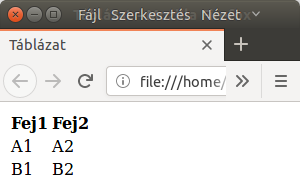
\includegraphics[width=\textwidth]{tabla1.png}
  \end{columns} 
\end{frame}

%41
\begin{frame}
  Szomszédos cellák (\texttt{<td>}, \texttt{<th>}) összevonásakor az összevont cellák száma
  \begin{description}[m]
    \item[vízszintes összevonásnál] \hfill \\ a bal szélső cella \texttt{colspan} attribútumában,
    \item[függőleges összevonásnál] \hfill \\ a legfelső cella \texttt{rowspan} attribútumában
  \end{description}
  van megadva. Az összevont cella tartalmát a bal szélső/legfelső cella elem tartalma adja meg. 
  A többi cella HTML elemét nem is adjuk meg!
\end{frame}

%42
\begin{frame}
  \begin{columns}[c]
    \column{0.7\textwidth}
      \begin{exampleblock}{\textattachfile{tabla21.html}{tabla21.html}, \textattachfile{tabla2.css}{tabla2.css}}
        \scriptsize
        \lstinputlisting[style=HTML,linerange={9-21},numbers=left,firstnumber=9]{tabla21.html}
      \end{exampleblock}
    \column{0.25\textwidth}
      \centering 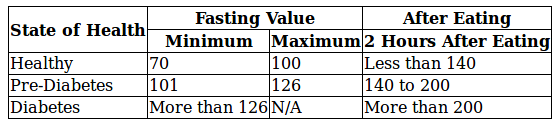
\includegraphics[width=\textwidth]{tabla21.png}
  \end{columns} 
\end{frame}

%43
\begin{frame}
  \begin{columns}[c]
    \column{0.6\textwidth}
      Készítse el az ábra alapján a \texttt{tabla22.html} fájlt! A cellák szegélyeinek megrajzolása érdekében 
      \begin{enumerate}
        \item ágyazza be a következő sort a \texttt{<head>} elembe:\\
          \texttt{<link rel="stylesheet" type="text/css" href="tabla2.css" />}
        \item Mentse ugyanabba a mappába a \texttt{tabla2.css} fájlt!
      \end{enumerate}
    \column{0.35\textwidth}
      \begin{exampleblock}{\textattachfile{tabla22.html}{tabla22.html}, \textattachfile{tabla2.css}{tabla2.css}}
        \centering 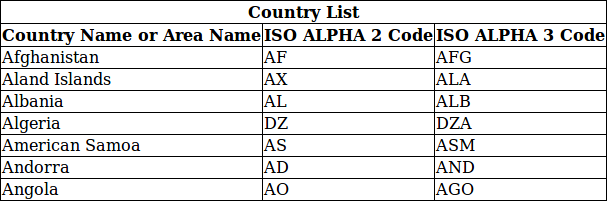
\includegraphics[width=\textwidth]{tabla22.png}
      \end{exampleblock}
  \end{columns} 
\end{frame}

%44
\begin{frame}
  Opcionális elemek, a \texttt{<table>}-be ágyazva:
  \begin{description}[m]
    \item[\texttt{<caption>}] \hfill \\ Táblázat címét adja meg (felül, középre igazítva)
    \item[\texttt{<colgroup>}] \hfill \\ Oszlopcsoport kialakítása, hogy az oszlopok azonos módon formázhatóak legyenek
    \item[\texttt{<col>}] \hfill \\ \texttt{<colgroup>}-ba ágyazandó, az oszlop formázásának megadásához. Azonosan 
      formázandó szomszédos oszlopoknak elég egy ilyen elem, a \texttt{span} attribútum adja meg az oszlopok számát.
  \end{description}
\end{frame}

%45
\begin{frame}
  További opcionális elemek:
  \begin{description}[m]
    \item[\texttt{<thead>}] \hfill \\ A fejléc sorainak (\texttt{<tr>}) egységbe zárására.
    \item[\texttt{<tbody>}] \hfill \\ A törzs részt zárja egybe.
    \item[\texttt{<tfoot>}] \hfill \\ A lábléc sorait zárja egybe.
  \end{description}
  Ezek a részek egységesen formázhatók, hosszú táblázatoknál a fej/láb minden oldalon újra kinyomtatható, 
  esetleg a törzs görgethető.\\
  Sorrend fontos: \texttt{<caption>} $\to$ \texttt{<colgroup>} $\to$ \texttt{<thead>} $\to$ \texttt{<tbody>} $\to$ \texttt{<tfoot>}
\end{frame}

%46
\begin{frame}
  \begin{columns}[c]
    \column{0.55\textwidth}
      \begin{exampleblock}{\textattachfile{tabla31.html}{tabla31.html}}
        \tiny
        \lstinputlisting[style=HTML,linerange={9-31},numbers=left,firstnumber=9]{tabla31.html}
      \end{exampleblock}
    \column{0.4\textwidth}
      \centering 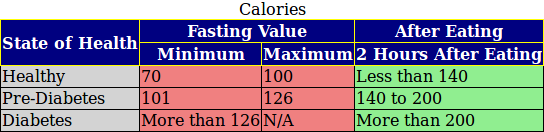
\includegraphics[width=\textwidth]{tabla31.png}
      \begin{exampleblock}{\textattachfile{tabla31.css}{tabla31.css}}
        \tiny
        \lstinputlisting{tabla31.css}
      \end{exampleblock}
  \end{columns} 
\end{frame}

%47
\begin{frame}
  \begin{columns}[c]
    \column{0.6\textwidth}
      Készítse el a \texttt{tabla22.html} átalakításával az ábra alapján a \texttt{tabla32.html} fájlt! 
      A megfelelő formázás érdekében 
      \begin{enumerate}
        \item cserélje le a korábbi \texttt{<link>} elemet a következőre:\\
          \texttt{<link rel="stylesheet" type="text/css" href="tabla32.css" />}
        \item Mentse ugyanabba a mappába a \texttt{tabla32.css} fájlt!
        \item Az első oszlop \texttt{<col>} elemének \texttt{class} attribútuma 
          legyen \texttt{country}, az utolsó kettőé \texttt{code} értékű!
      \end{enumerate}
    \column{0.35\textwidth}
      \begin{exampleblock}{\textattachfile{tabla32.html}{tabla32.html}, \textattachfile{tabla32.css}{tabla32.css}}
        \centering 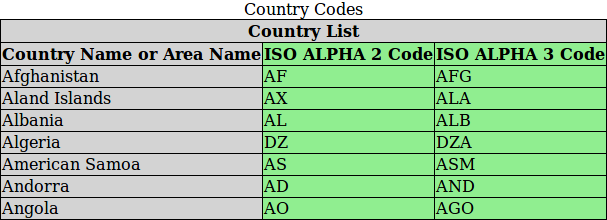
\includegraphics[width=\textwidth]{tabla32.png}
      \end{exampleblock}
  \end{columns} 
\end{frame}

%48
\begin{frame}
  \begin{columns}[c]
    \column{0.24\textwidth}
      \footnotesize
      Táblázat beágyazható egy másik táblázat (fejléc) cellájába. Előnye: a cellák mérete, 
      oszlopok száma táblázatonként eltérő lehet.\\
      \medskip
      \centering 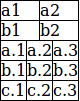
\includegraphics[scale=.75]{tabla4.png}
    \column{0.71\textwidth}
      \begin{exampleblock}{\textattachfile{tabla4.html}{tabla4.html}, \textattachfile{tabla4.css}{tabla4.css}}
        \scriptsize
        \lstinputlisting[style=HTML,linerange={9-23},numbers=right,firstnumber=9]{tabla4.html}
      \end{exampleblock}
  \end{columns} 
\end{frame}
